\documentclass[a4paper]{article}

\usepackage{fontspec}
\usepackage{tikz}
\usetikzlibrary{calc}
\usepackage[dvipsnames]{xcolor}

\definecolor{mygray}{gray}{0.6}
\setmainfont{SFUIDisplay-Light.ttf}

\date{}

\begin{document}
\maketitle

\begin{tikzpicture}[overlay, remember picture]
\node[anchor=north west,
      xshift=16.5cm,
      yshift=-28.4cm] 
     at (current page.north west) 
     {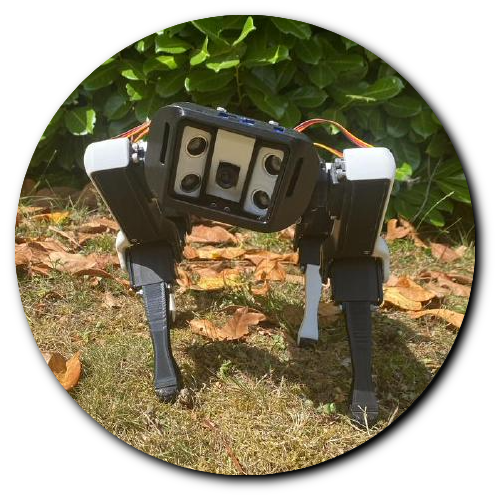
\includegraphics[width=0.7cm]{shadowed_example_pfp.png}}; 
\end{tikzpicture}

\begin{tikzpicture}[overlay]
    \foreach \x in {-8,...,30}
    \foreach \y in {-40,...,15}
    { \fill[gray!75] (0.5*\x,0.5*\y) circle (0.03cm); }       
\end{tikzpicture}

\setlength{\footskip}{100pt}

\renewcommand{\thepage}{\scriptsize{Supporting open source. Visit \url{https://github.com/vertueux/prototyping-papers} for the copy and use of this paper.}}

\end{document}